% !TEX program = pdflatex
% Concise, rubric-ordered Part 3 report. Long version with every bench and debug note:
% ESE5700_Proj1_Part3.tex. Cropped figures in img/short/ (falls back to img/).
\documentclass[10pt,letterpaper]{article}
\usepackage[T1]{fontenc}
\usepackage{lmodern,amsmath,amssymb,booktabs,graphicx,microtype,array,tabularx}
\usepackage[margin=.7in,headheight=14pt]{geometry}
\usepackage{float,xcolor,fancyhdr,colortbl,tikz,caption}
\usetikzlibrary{arrows.meta,automata,positioning}
\usepackage[colorlinks=true,linkcolor=blue!40!black,urlcolor=blue!40!black]{hyperref}
\definecolor{navy}{HTML}{153654}\definecolor{pale}{HTML}{EAF1F7}
\setlength{\parindent}{0pt}\setlength{\parskip}{3pt}
\graphicspath{{img/short/}{img/}}
\pagestyle{fancy}\fancyhf{}\fancyhead[L]{\small ESE 5700 / Project 1 / Part 3}\fancyhead[R]{\small MAC unit (concise)}\fancyfoot[C]{\thepage}\renewcommand{\headrulewidth}{.3pt}
\captionsetup{font=small,labelfont=bf,skip=2pt}
\newcommand{\todo}[1]{\textcolor{red}{\textbf{[TODO: #1]}}}
\newcommand{\code}[1]{\texttt{#1}}
\newcommand{\fig}[3]{\begin{figure}[H]\centering\includegraphics[width=#2\linewidth]{#1}\caption{#3}\end{figure}}
\newcommand{\twofig}[4]{\begin{figure}[H]\centering\raisebox{-.5\height}{\includegraphics[width=.49\linewidth,height=.25\textheight,keepaspectratio]{#1}}\hfill\raisebox{-.5\height}{\includegraphics[width=.49\linewidth,height=.25\textheight,keepaspectratio]{#2}}\caption{#3}\label{#4}\end{figure}}
\begin{document}
\begin{center}
{\small UNIVERSITY OF PENNSYLVANIA \quad ESE 5700}\par\vspace{3pt}
{\LARGE\bfseries Project 1, Part 3: the MAC unit}\par\vspace{2pt}
Tyrone Marhguy \quad\textbullet\quad Victor Wanjohi\par\vspace{3pt}
\colorbox{pale}{\parbox{.96\linewidth}{\small\centering Cadence GPDK 18 nm \quad $V_{DD}=0.8$ V, TT, 27$^\circ$C \quad schematic level, $C_{BL}=3.5$ fF \quad Tests A, B, C pass \quad 17 cycles START$\to$DONE \quad area $\approx290\ \mu$m$^2$ (est.) \quad $T_{CLK,\min}=\todo{}$}}
\end{center}

\section*{1. Team and architecture}
\begin{tabularx}{\linewidth}{@{}lX@{}}\toprule Member & Contribution\\\midrule
Tyrone Marhguy & \todo{fill in}\\
Victor Wanjohi & \todo{fill in}\\\bottomrule\end{tabularx}

Two Part 2 macros hold $W$ and $X$; a static-CMOS array multiplier, a 12-bit ripple accumulator, a 4-bit counter and a two-state-bit controller (all registers are transmission-gate master--slave flip-flops) compute $\mathrm{ACC}=\sum_{i=0}^{15}W[i]X[i]$. The read is pipelined against the multiply-accumulate: the macro's output latch is the only pipeline stage, so a dot product takes 17 cycles.
\twofig{mac_top_schematic}{mac_top_schematic_right}{\code{top}. Left: macros (WE $=$ LOAD\_EN$\cdot$WE\_W / WE\_X), multiplier, accumulator, LOAD\_EN $=\overline{\mathrm{RUN}+\mathrm{DONE}+\mathrm{START}}$. Right: controller, counter, address mux (COUNT while RUN).}{fig:top}

\section*{2. Register (3.1)}
Positive-edge master--slave flip-flop from two static TG latches (master transparent while CLK $=0$, slave while CLK $=1$); \code{tg} 2+2 fins, \code{inv\_2x} 8/4 fins, 100 fins. Chosen because it is fully static (holds with the clock stopped), needs one clock, and reuses verified cells; the cost is two local clock inverters (clock load). \code{register\_1b} adds a \code{mux2} enable and an \code{and2} synchronous reset (RST active-high), 152 fins.
\twofig{dff_schematic}{tb_dff_close_graph}{\code{d\_ff} (left) and \code{tb\_dff}: Q captures on each rising CLK, $t_{cq}\approx100$ ps (CLK 50\% $\to$ Q 50\%, $C_Q=1$ fF).}{fig:dff}
\begin{center}\small\begin{tabular}{@{}lll@{}}\toprule Quantity & Value & Simulation\\\midrule
$t_{cq}$ (rise/fall) & 100 ps & \code{tb\_dff}, D stable 1 ns before the edge\\
$t_{su}$ / $t_h$ & \todo{} / \todo{} & D-to-CLK offset sweep, 10\% $t_{cq}$ push-out\\
$C_{CLK}$ & \todo{} fF & CLK-source charge per cycle $/V_{DD}$\\
Energy per clock & \todo{} fJ & $\int V_{DD}I_{DD}\,dt$ over one cycle\\\bottomrule\end{tabular}\end{center}

\section*{3. Datapath (3.2)}
\textbf{Multiplier:} 16 \code{and2} partial products and three 4-bit ripple rows (12 full adders, 2096 fins). \textbf{Accumulator:} 12-bit ripple adder ($B=\{0000,P\}$, $3600<4096$) into 12 \code{register\_1b} (3600 fins). Full adder: 2 \code{xor2} (static, input inverters; NMOS 2/4, PMOS 2 fins), 2 \code{and2}, 1 \code{or2}, 148 fins.
\twofig{mult4x4_schematic}{adder12_schematic}{\code{multiplier4b} (row $j$ ANDs $A$ with $B_j$) and \code{fulladder\_12b}.}{fig:dp}

\textbf{Logical effort} ($\tau=10.5$ ps from Part 2 FO4 $=53$ ps; $f$ from fin ratios to \code{inv\_u}, worst edge):
\begin{center}\small\begin{tabular}{@{}lr@{\qquad}lr@{}}\toprule Full-adder arc & $d$ & Path & Delay\\\midrule
$C_{in}\to C_{out}$ & $17\tau$ & multiplier: and2, $3\times$($A/B\to C_{out}$, $C_{in}\to S$), 3 carries to $P_7$ & $176\tau=1.85$ ns\\
$C_{in}\to S$ & $13\tau$ & accumulator: $P_4$, carries to bit 11 & $145\tau=1.5$ ns\\
$A/B\to S$ & $26\tau$ & register input (\code{mux2}+\code{and2}) & 0.1 ns\\
$A/B\to C_{out}$ & $30\tau$ & & \\\bottomrule\end{tabular}\end{center}
The \code{xor2} core dominates: its 2-fin series PMOS stack is $\approx4\times$ weaker than \code{inv\_u} (12 of the $26\tau$ of a sum arc). Upsizing it to 4-fin stacks would cut the multiplier to $\approx1.3$ ns (LE).

\textbf{Exhaustive multiplier test:} all 256 pairs; the check samples $|P-A\cdot B|$ at $0.95\,t_v$ in every vector (spec $<0.5$).
\begin{center}\small\begin{tabular}{@{}lcccccc@{}}\toprule $t_v$ (ns) & 1.0 & 1.1 & 1.2 & \textbf{1.3} & 1.4 & 1.5\\\midrule
errmax & 44 & 14 & 0.62 & \textbf{0.17} & 0.14 & 0.12\\ result & fail & fail & fail & \textbf{pass} & pass & pass\\\bottomrule\end{tabular}\end{center}
256/256 correct; \textbf{measured worst case 1.2 ns} (1.14--1.24 ns; vector $B=15$, $A$ $3\to4$) against \textbf{1.85 ns predicted}: LE charges every stage its slow edge and the full load.
\fig{tb_multiplier4b_errS}{.62}{Sampled error at $t_v=1$ ns: zero except a few carry-heavy vectors still settling at 0.95 ns.}

\section*{4. Sequencer (3.3)}
\begin{minipage}[t]{.42\linewidth}\vspace{0pt}\centering
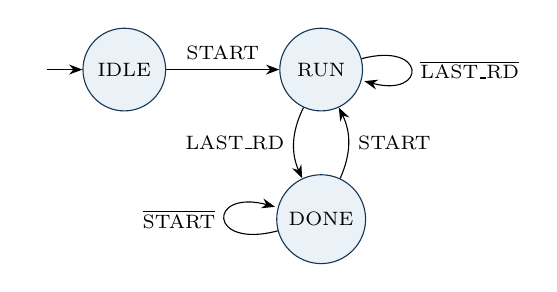
\begin{tikzpicture}[->,>=Stealth,node distance=2.5cm,auto,every state/.style={fill=pale,draw=navy,minimum size=1.05cm,font=\scriptsize}]
\node[state,initial,initial text=] (idle) {IDLE};
\node[state,right of=idle] (comp) {RUN};
\node[state,below of=comp,node distance=1.9cm] (done) {DONE};
\path (idle) edge node {\scriptsize START} (comp)
      (comp) edge[loop right] node {\scriptsize $\overline{\mathrm{LAST\_RD}}$} ()
      (comp) edge[bend right=25,swap] node[left] {\scriptsize LAST\_RD} (done)
      (done) edge[bend right=25,swap] node[right] {\scriptsize START} (comp)
      (done) edge[loop left] node {\scriptsize $\overline{\mathrm{START}}$} ();
\end{tikzpicture}\end{minipage}\hfill
\begin{minipage}[t]{.56\linewidth}\vspace{0pt}\small
State $(S_0,\mathrm{DONE})$; RUN $=S_0\overline{\mathrm{DONE}}$. START (not in RUN) raises CLEAR (ACC, counter) and sets $S_0$. In RUN: COUNT\_EN $=\overline{\mathrm{LAST}}$ (count 0--15, hold at 15), ACC\_EN $=$ VALID (RUN one cycle late: pipeline). LAST\_READ, set the cycle after count $=15$, ends RUN and sets DONE, which holds until START. RST clears all. Counter: synchronous toggle chain, 4 \code{d\_ff}.\end{minipage}
\twofig{counter4b_schematic}{controller_schematic_logic}{\code{counter\_4b} and \code{controller\_mac} next-state logic (state registers in the long report).}{fig:seq}
\fig{tb_controller_tran}{.9}{\code{controller\_mac}$+$\code{counter\_4b}, vector-file bench (60 edges, \textbf{60/60 checks pass}; counter alone 38/38): START at edge 5, DONE after edge 22 (\textbf{17 edges}), restart from DONE, START ignored in RUN, RST abort, full second run.}
\textbf{One dot product (Test A, $T=10$ ns):} START edge 332 ns $\to$ RUN, count 0; edge $n$ reads address $n-1$ and DOUT is valid $\approx0.5$ ns later; ACC\_EN from 342 ns, first accumulate at 352 ns; 16th at 502 ns with DONE (Fig.~\ref{fig:testA}). \todo{Drawn timing diagram.}

\section*{5. Timing closure (3.4)}
Critical path (one stage after the macro's output latch): CLK $\to$ SRAM access $\to$ multiplier $\to$ adder $\to$ register setup.
\begin{center}\small\begin{tabular}{@{}lll@{}}\toprule Term & Value & Source\\\midrule
$t_{\text{SRAM}}$ & 0.49 ns & Part 2 worst-case access\\
$t_{\text{mult}}$ & 1.85 ns LE / 1.2 ns measured & \S3\\
$t_{\text{add}}+$ register input & 1.6 ns LE & \S3\\
$t_{su}$ & \todo{} & \S2\\\midrule
\textbf{Hand $T_{\min}$} & \textbf{4.0 ns} $+\,t_{su}$ (3.3 ns with the measured multiplier) & sum\\
\textbf{Measured $T_{\min}$} & \todo{} & shortest $T$ at which A, B, C pass\\\bottomrule\end{tabular}\end{center}
\textbf{Hold:} counter $\to$ \code{mux2} $\to$ macro address latch, which closes at the same edge; requires $t_{cq,\min}+t_{\text{mux}}>t_{h}$. \todo{margin}

\section*{6. Verification (3.5)}
Vector-file stimulus: reset, load $W$ then $X$ (one word per cycle, inputs change on the falling edge), START, run, $T=10$ ns.
\begin{center}\small\begin{tabular}{@{}llllc@{}}\toprule Test & $W$, $X$ & Expected & ACC & Result\\\midrule
A & handout vectors & 845 (0x34D) & 0x34D & \textbf{pass}\\
B & all 15 & 3600 (0xE10) & 0xE10 & \textbf{pass}\\
C & 5/10 alternating & 800 (0x320) & 0x320 & \textbf{pass}\\\bottomrule\end{tabular}\end{center}
DONE rises 17 edges after START in all three. \textbf{Bug found here:} ACC first read 0 because the macro's output-latch enable was a 150 ps pulse that closed before the read inverter switched; it is now level-sensitive on CLK high (RD\_EN $=\mathrm{CLKBUF}\cdot\overline{\mathrm{WE\_L}}$).
\begin{figure}[H]\centering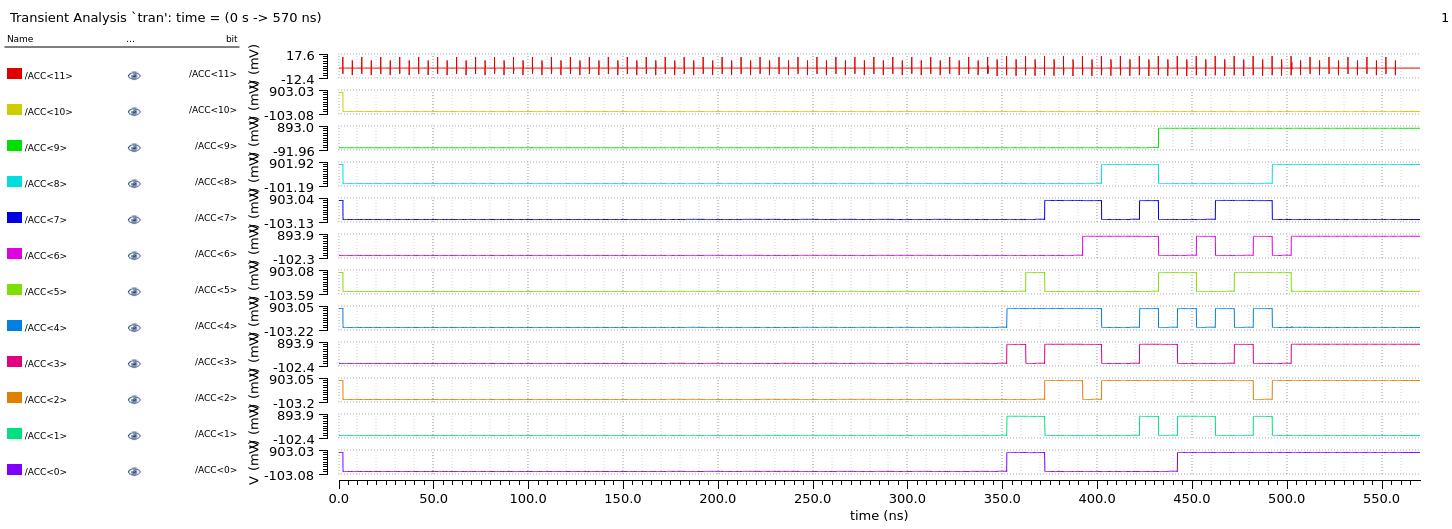
\includegraphics[width=.92\linewidth]{tb_top_testA_acc}\caption{\textbf{Test A}: ACC steps 27, 51, 156, \ldots, 805, \textbf{845 (0x34D)} at 502 ns and holds. \todo{add DONE trace}}\label{fig:testA}\end{figure}
\fig{tb_top_rden_bug}{.7}{Before the fix: RD rises after the read, but the RD\_EN pulse closes first; the latch node X peaks near 0.4 V and returns to 0.}

\section*{7. Metrics}
\begin{center}\small\begin{tabular}{@{}ll@{}}\toprule Metric & Value\\\midrule
$T_{CLK,\min}$; $N_{cycles}$; $t_{dot}$ & \todo{}; 17; \todo{}\\
Area (2 macros $+$ datapath 5696 fins $+$ sequencer 1848 fins, $D=28$) & $109+138+45\approx290\ \mu$m$^2$ (est.)\\
$E_{dot}$ (Test A/B/C); energy per MAC with / without memory & \todo{}\\
FOM$_{MAC}$ $=$ Area$\cdot E_{dot}\cdot t_{dot}$ & \todo{}\\\bottomrule\end{tabular}\end{center}

\section*{8. What limited the design}
The multiply-accumulate path, not the memory, sets the clock: the ripple multiplier alone takes 1.2 ns, over twice the 0.49 ns SRAM read, before the ripple adder and setup. Both use one small full adder whose 2-fin \code{xor2} stacks dominate the delay; the datapath is also the largest area (138 $\mu$m$^2$, more than both macros). Next steps: carry-save multiplier, carry-select final adder, upsized \code{xor2}, and a register after the multiplier (18 cycles, within the 20-cycle limit). \todo{energy}
\end{document}
